% https://github.com/svmiller/svm-r-markdown-templates

\documentclass[11pt,]{article}
\usepackage[left=1in,top=1in,right=1in,bottom=1in]{geometry}
\newcommand*{\authorfont}{\fontfamily{phv}\selectfont}
\usepackage[]{libertine}


  \usepackage[T1]{fontenc}
  \usepackage[utf8]{inputenc}




\usepackage{abstract}
\renewcommand{\abstractname}{}    % clear the title
\renewcommand{\absnamepos}{empty} % originally center

\renewenvironment{abstract}
 {{%
    \setlength{\leftmargin}{0mm}
    \setlength{\rightmargin}{\leftmargin}%
  }%
  \relax}
 {\endlist}

\makeatletter
\def\@maketitle{%
  \newpage
%  \null
%  \vskip 2em%
%  \begin{center}%
  \let \footnote \thanks
    {\fontsize{18}{20}\selectfont\raggedright  \setlength{\parindent}{0pt} \@title \par}%
}
%\fi
\makeatother




\setcounter{secnumdepth}{0}


\usepackage{graphicx,grffile}
\makeatletter
\def\maxwidth{\ifdim\Gin@nat@width>\linewidth\linewidth\else\Gin@nat@width\fi}
\def\maxheight{\ifdim\Gin@nat@height>\textheight\textheight\else\Gin@nat@height\fi}
\makeatother
% Scale images if necessary, so that they will not overflow the page
% margins by default, and it is still possible to overwrite the defaults
% using explicit options in \includegraphics[width, height, ...]{}
\setkeys{Gin}{width=\maxwidth,height=\maxheight,keepaspectratio}


\title{Analysis Plan: Replicating Growth and Inequality in Public Good
Provision \thanks{Further replication files are available on the
author's Github account (\url{http://github.com/howquez}).
\textbf{Current version}: February 01, 2022; \textbf{Corresponding
author}:
\href{mailto:roggenkh@hsu-hh.de}{\nolinkurl{roggenkh@hsu-hh.de}}.}  }
 



\author{\Large Hauke
Roggenkamp\vspace{0.05in} \newline\normalsize\emph{Helmut-Schmidt-University}   \and \Large Stefan
Traub\vspace{0.05in} \newline\normalsize\emph{Helmut-Schmidt-University}   \and \Large Michael
Berlemann\vspace{0.05in} \newline\normalsize\emph{Helmut-Schmidt-University}  }


\date{}

\usepackage{titlesec}

\titleformat*{\section}{\normalsize\bfseries}
\titleformat*{\subsection}{\normalsize\itshape}
\titleformat*{\subsubsection}{\normalsize\itshape}
\titleformat*{\paragraph}{\normalsize\itshape}
\titleformat*{\subparagraph}{\normalsize\itshape}


\usepackage{natbib}
\bibliographystyle{apsr}
\usepackage[strings]{underscore} % protect underscores in most circumstances



\newtheorem{hypothesis}{Hypothesis}
\usepackage{setspace}


% set default figure placement to htbp
\makeatletter
\def\fps@figure{htbp}
\makeatother

\usepackage{hyperref}
\usepackage{array}
\usepackage{caption}
\usepackage{graphicx}
\usepackage{siunitx}
\usepackage[table]{xcolor}
\usepackage{multirow}
\usepackage{hhline}
\usepackage{calc}
\usepackage{tabularx}
\usepackage{fontawesome}
\usepackage[para,online,flushleft]{threeparttable}

% move the hyperref stuff down here, after header-includes, to allow for - \usepackage{hyperref}

\makeatletter
\@ifpackageloaded{hyperref}{}{%
\ifxetex
  \PassOptionsToPackage{hyphens}{url}\usepackage[setpagesize=false, % page size defined by xetex
              unicode=false, % unicode breaks when used with xetex
              xetex]{hyperref}
\else
  \PassOptionsToPackage{hyphens}{url}\usepackage[draft,unicode=true]{hyperref}
\fi
}

\@ifpackageloaded{color}{
    \PassOptionsToPackage{usenames,dvipsnames}{color}
}{%
    \usepackage[usenames,dvipsnames]{color}
}
\makeatother
\hypersetup{breaklinks=true,
            bookmarks=true,
            pdfauthor={Hauke
Roggenkamp (Helmut-Schmidt-University) and Stefan
Traub (Helmut-Schmidt-University) and Michael
Berlemann (Helmut-Schmidt-University)},
             pdfkeywords = {dynamic public goods game, inequality,
cooperation, growth},  
            pdftitle={Analysis Plan: Replicating Growth and Inequality
in Public Good Provision},
            colorlinks=true,
            citecolor=blue,
            urlcolor=blue,
            linkcolor=magenta,
            pdfborder={0 0 0}}
\urlstyle{same}  % don't use monospace font for urls

% Add an option for endnotes. -----


% add tightlist ----------
\providecommand{\tightlist}{%
\setlength{\itemsep}{0pt}\setlength{\parskip}{0pt}}

% add some other packages ----------

% \usepackage{multicol}
% This should regulate where figures float
% See: https://tex.stackexchange.com/questions/2275/keeping-tables-figures-close-to-where-they-are-mentioned
\usepackage[section]{placeins}


\begin{document}
	
% \pagenumbering{arabic}% resets `page` counter to 1 
%    

% \maketitle

{% \usefont{T1}{pnc}{m}{n}
\setlength{\parindent}{0pt}
\thispagestyle{plain}
{\fontsize{18}{20}\selectfont\raggedright 
\maketitle  % title \par  

}

{
   \vskip 13.5pt\relax \normalsize\fontsize{11}{12} 
\textbf{\authorfont Hauke
Roggenkamp} \hskip 15pt \emph{\small Helmut-Schmidt-University}   \par \textbf{\authorfont Stefan
Traub} \hskip 15pt \emph{\small Helmut-Schmidt-University}   \par \textbf{\authorfont Michael
Berlemann} \hskip 15pt \emph{\small Helmut-Schmidt-University}   

}

}








\begin{abstract}

    \hbox{\vrule height .2pt width 39.14pc}

    \vskip 8.5pt % \small 

\noindent We replicate a public goods experiment with dynamic
interdependency and find similar results as GMTV. Absolute contributions
increase over time. Just as in static public goods experiments, the
share of endowments contributed decreases over time. The richest groups
earn fifteen times more than the poorest groups. While there clearly is
growth, groups do not realize the maximal potential efficiency and earn
just a fraction of what is possible. Even though we conducted the
experiment online and remotely, dropouts are no concern. Participants
make relatively fast decisions which makes longer games feasible in the
future. Taken together with inefficient growth and the lack of dropouts,
additional rounds are fairly cheap.


\vskip 8.5pt \noindent \emph{Keywords}: dynamic public goods game,
inequality, cooperation, growth \par

    \hbox{\vrule height .2pt width 39.14pc}



\end{abstract}


\vskip -8.5pt


 % removetitleabstract

\noindent  

\hypertarget{background}{%
\section{Background}\label{background}}

In an attempt to incorporate uncertainty to \citet{GMTV2017}'s dynamic
public goods game (DPGG), I plan to run a series of remote online
experiments using oTree \citep{oTree}. This experiment replicated
Gächter et al.'s NOPUNISH 10-round treatment arm as close as possible
(given the remote circumstances). The current demo version of the
experiment can be found \href{https://cliccs.herokuapp.com/}{here}.
Click \href{https://github.com/Howquez/coopUncertainty}{here} to visit
the corresponding Github repository.

\href{https://github.com/Howquez/coopUncertainty/blob/July21Replication/analysis/reports/rmd/03_dataAnalyses.Rmd}{This
report} is the third in a series of reports covering this project. It
reads the data prepared in the previous reports and analyzes them. The
whole replication project is registered in the AEA RCT Registry and the
unique identifying number is:
\href{https://doi.org/10.1257/rct.7902-2.0}{AEARCTR-0007902}
\citep{preregistration}.

\hypertarget{data}{%
\section{Data}\label{data}}

I'll refer to the data \citet{GMTV2017} provided as \emph{GMTV} or
\emph{noPunish10} in what follows. GMTV conducted most of their sessions
in late 2012. All of these sessions ran in Nottingham using a student
sample. collected They 23 observations in their NOPUNISH 10 treatment
arm. Our data, refered to as \emph{replication} is more recent, gathered
remotely in Hamburg using a different tech stack as well as a different
sample.

We conducted a series a 4 sessions in between Thursday, July 01 to
Friday, July 23 2021 and collected 29 observations (from 116
participants) in total. 35 additional participants could not be matched
with other group members or failed to answer the comprehension
questions. These participants are labeled as dropouts. None of them
dropped out during the session such that attrition is no problem here.

Two of these sessions were special: The first (jyf8xd0s) as well as the
last one (d6jrsxnr). The first session suffered technical problems such
that the risk elicitation task was omitted. The last session (almost
exclusively) relied on a student sample as our non-student sample was
exhausted after the first three sessions. As a consequence, the last
session was conducted with 59 students while all others were conducted
without any students. I'll therefore create a boolean \texttt{student}
variable.

All participants were recruited in by the University of Hamburg's WISO
Research Lab using HROOT \citep{hroot}.

\hypertarget{results}{%
\section{Results}\label{results}}

\hypertarget{first-round}{%
\subsection{First Round}\label{first-round}}

We start by discussing initial contributions which assume the full range
between 0 and 20 as Table 1 illustrates. Both the median as well as the
mean are about 10 tokens, that is, 50\% of the initial endowment in both
data sources. This is comparable to initial contributions in the
standard game with partner matching.\footnote{See Figure 3B in
  \citet{fehrgaechter2000}, for instance.}

\begin{table}[!htbp] \centering 
  \caption{} 
  \label{} 
\begin{tabular}{@{\extracolsep{5pt}}lcc} 
\\[-1.8ex]\hline 
\hline \\[-1.8ex] 
Statistic & replication & GMTV \\ 
\hline \\[-1.8ex] 
Mean & 10.017 & 10.685 \\ 
Median & 10 & 10.000 \\ 
St. Dev. & 6.340 & 5.881 \\ 
Max & 20 & 20.000 \\ 
Min & 0 & 0.000 \\ 
N & 116 & 92 \\ 
\hline \\[-1.8ex] 
\end{tabular} 
\end{table}

The two-sided rank sum test (comparing differences between data sources)
yields a p-Value of 0.3926 for the mean contribution in first round of
the game.

\hypertarget{provision-of-the-public-good}{%
\subsection{Provision of the public
good}\label{provision-of-the-public-good}}

We proceed by further discussing contributions. The left panel in Figure
1 shows the average amount of tokens participants contributed over time.
Contributions are clearly non-zero and are increasing over time in the
replication treatment.\footnote{Participants contribute about 10 tokens
  in the first round} While contributions flatten in the replication,
the GMTV data exhibit a drop in the last round. Note that increasing
contributions over time imply that participants have increasing
endowments over time. Hence, increasing contributions do not necessarily
imply that participants contribute increasing shares of their
endowments. The right panel in Figure 1 shows the share of overall
endowments contributed over time. In the original data, participants
contribute around 53\% of their endowment in round 1. This amount
steadily decreases. The replication exhibits a similar pattern with an
initial average contributions of 50\%. Both treatments resemble the
results from the standard game: Just as in \citet{fehrgaechter2000}
contributions start at a level of around 50-60\% of endowments and
decrease to around 10\% of endowments in round 10.

\begin{figure}
\centering
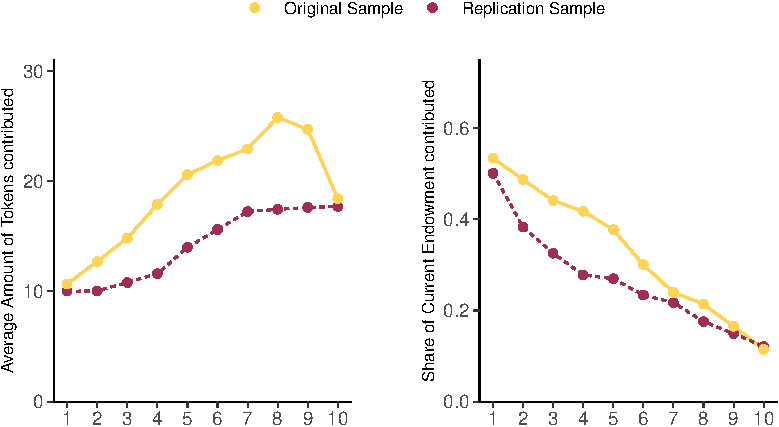
\includegraphics{/Users/hauke.roggenkamp/Documents/dev/coopUncertainty/analysis/reports/prettyReports/04_Analyses_files/figure-latex/plotShareOfContributions-1.pdf}
\caption{The average amount of tokens contributed over time in
treatments.}
\end{figure}

\hypertarget{wealth-creation}{%
\subsection{Wealth Creation}\label{wealth-creation}}

Possibly of more interest are the implications contributions have for
wealth generation and growth. To measure growth, we define a variable
\emph{stock} which sums the endowments of all participants in a given
group at the end of the round (that is, after the contributions have
been made, multiplied and redistributed). \citet{GMTV2017} refer to that
variable as ``wealth'' so we will do the same in what follows. Before
the start of round 1, wealth will be 80 in all groups by construction.
The maximal wealth that can be reached in round 10 (if everyone
contributes their entire endowment in each round) is approximately 4613
tokens or 230 Euro per group. Table 3 shows some summary statistics
regarding wealth. Groups do achieve growth on average. While there is
clearly growth, groups do not realize the maximal potential efficiency
as the replication groups reach on average a level of 379 tokens out of
4613 maximally possible or 8.2\%. As in the original data, there is
large heterogeneity with the richest group reaching 1425 tokens whereas
the poorest group ends up with 92 tokens.

\begin{figure}
\centering
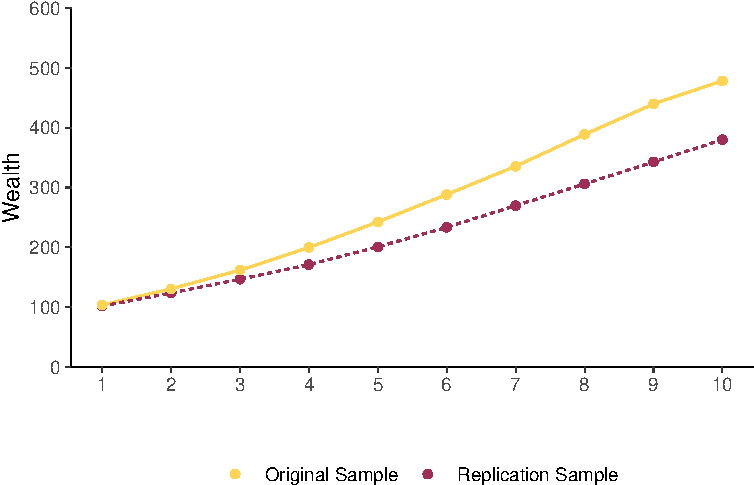
\includegraphics{/Users/hauke.roggenkamp/Documents/dev/coopUncertainty/analysis/reports/prettyReports/04_Analyses_files/figure-latex/plotStock-1.pdf}
\caption{Average wealth over time across treatments.}
\end{figure}

Figure 2 shows the dynamics of wealth over time. The left panel focuses
on all groups, the upper right panel on those with above median wealth
after round 10 (``successful'' groups) and the lower left panel on those
with below median wealth after round 10 (``unsuccessful'' groups). The
average wealth is increasing across rounds and is substantially above 80
once round 10 was played as Table 2 illustrates.

\begin{table}[!htbp] \centering 
  \caption{} 
  \label{} 
\begin{tabular}{@{\extracolsep{5pt}}lcc} 
\\[-1.8ex]\hline 
\hline \\[-1.8ex] 
Statistic & replication & GMTV \\ 
\hline \\[-1.8ex] 
Mean & 379.828 & 478.087 \\ 
Median & 262 & 304.000 \\ 
St. Dev. & 336.059 & 393.575 \\ 
Max & 1,425 & 1,792.000 \\ 
Min & 92 & 161.000 \\ 
N & 29 & 23 \\ 
\hline \\[-1.8ex] 
\end{tabular} 
\end{table}

The two-sided rank sum test (comparing differences between data sources)
yields a p-Value of 0.1356 for the mean wealth after the last round of
the game.

\hypertarget{wealth-differences-between-data-sources}{%
\subsubsection{Wealth Differences between Data
Sources}\label{wealth-differences-between-data-sources}}

We next consider whether we were able to replicate GMTV's results with
our data. Absolute contributions tended to be higher in \citet{GMTV2017}
but end up at around the same level as in the replication due to a stark
decline in contributions on the last round. In terms of shares
contributed both data sources exhibit a similar pattern: they decline
and do not stabilize. Even though the share of current endowments
contributed in the last round is quite similar, the share declined a
little faster in our data.

Our groups also tend to be poorer. Median wealth is higher in GMTV. This
difference in mean ranks is not significant according to a two-sided
ranksum test, however. To assess the statistical significance of
differences in means, we run OLS regressions where we regress wealth on
a treatment dummy for \emph{Replication} (Table 3). These regressions
show that differences in means are only significant for below median
groups.

\begin{table}[!htbp] \centering 
  \caption{} 
  \label{} 
\begin{tabular}{@{\extracolsep{5pt}}lccc} 
\\[-1.8ex]\hline 
\hline \\[-1.8ex] 
 & \multicolumn{3}{c}{\textit{Dependent variable:}} \\ 
\cline{2-4} 
\\[-1.8ex] & \multicolumn{3}{c}{Wealth} \\ 
 & All & Below median & Above median \\ 
\hline \\[-1.8ex] 
 Replication & $-$98.26 & $-$59.41$^{***}$ & $-$138.21 \\ 
  & (101.21) & (18.32) & (166.67) \\ 
  & & & \\ 
 Constant & 478.09$^{***}$ & 234.70$^{***}$ & 731.00$^{***}$ \\ 
  & (75.58) & (13.99) & (124.73) \\ 
  & & & \\ 
\hline \\[-1.8ex] 
Observations & 52 & 24 & 25 \\ 
R$^{2}$ & 0.02 & 0.32 & 0.03 \\ 
Residual Std. Error & 362.49 & 44.24 & 413.67 \\ 
\hline 
\hline \\[-1.8ex] 
\textit{Note:}  & \multicolumn{3}{r}{$^{*}$p$<$0.1; $^{**}$p$<$0.05; $^{***}$p$<$0.01} \\ 
\end{tabular} 
\end{table}

\hypertarget{inequality}{%
\subsection{Inequality}\label{inequality}}

In this subsection, we focus on the amount of inequality created
endogenously in our setting. The smallest possible value the Gini
coefficient takes is zero (if all four group members own one fourth of
the wealth) and the largest possible value it takes is one (if one group
member holds the entire wealth). Table 4 shows some summary statistics
regarding the Gini coefficient.

The round 10 Gini coefficient ranges between 0.035 and 0.52 in our data
with a median of 0.218.

\begin{table}[!htbp] \centering 
  \caption{} 
  \label{} 
\begin{tabular}{@{\extracolsep{5pt}}lcc} 
\\[-1.8ex]\hline 
\hline \\[-1.8ex] 
Statistic & replication & GMTV \\ 
\hline \\[-1.8ex] 
Mean & 0.218 & 0.246 \\ 
Median & 0.218 & 0.245 \\ 
St. Dev. & 0.123 & 0.131 \\ 
Max & 0.520 & 0.479 \\ 
Min & 0.035 & 0.044 \\ 
N & 29 & 23 \\ 
\hline \\[-1.8ex] 
\end{tabular} 
\end{table}

The two-sided rank sum test yields a p-Value of 0.4176 for the mean
\texttt{gini} during the last round of the game.

Figure 3 illustrates the dynamics of the Gini coefficient (at the end of
each round) over time and shows that inequality increases slightly.

\begin{figure}
\centering
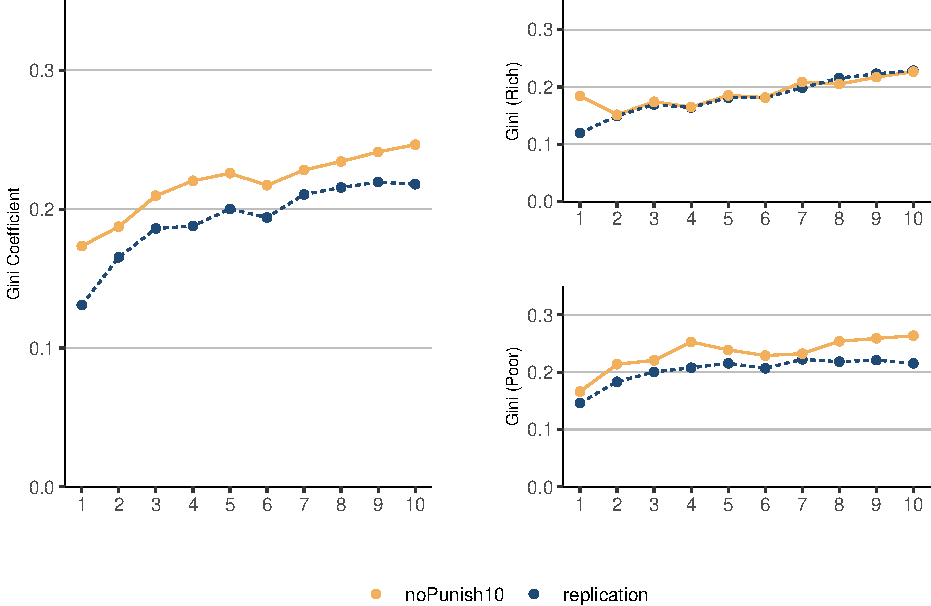
\includegraphics{/Users/hauke.roggenkamp/Documents/dev/coopUncertainty/analysis/reports/prettyReports/04_Analyses_files/figure-latex/plotInequality-1.pdf}
\caption{Average Gini coefficient over time across treatments.}
\end{figure}

\hypertarget{inequality-differences-between-data-sources}{%
\subsubsection{Inequality Differences between Data
Sources}\label{inequality-differences-between-data-sources}}

Once more, we consider whether we were able to replicate GMTV's results
with our data.

The following table shows a simple OLS regression to illustrate
differences in the 10th round's Gini coefficient between the
replication's data and GMTV's data. Mean Gini coefficients are similar
across data sources and there are no statistically significant
differences in mean Gini coefficients.

\begin{table}[!htbp] \centering 
  \caption{} 
  \label{} 
\begin{tabular}{@{\extracolsep{5pt}}lccc} 
\\[-1.8ex]\hline 
\hline \\[-1.8ex] 
 & \multicolumn{3}{c}{\textit{Dependent variable:}} \\ 
\cline{2-4} 
\\[-1.8ex] & \multicolumn{3}{c}{Gini} \\ 
 & All & Below median & Above median \\ 
\hline \\[-1.8ex] 
 Replication & $-$0.03 & $-$0.05 & 0.002 \\ 
  & (0.04) & (0.06) & (0.05) \\ 
  & & & \\ 
 Constant & 0.25$^{***}$ & 0.26$^{***}$ & 0.23$^{***}$ \\ 
  & (0.03) & (0.04) & (0.04) \\ 
  & & & \\ 
\hline \\[-1.8ex] 
Observations & 52 & 24 & 25 \\ 
R$^{2}$ & 0.01 & 0.03 & 0.0001 \\ 
Residual Std. Error & 0.13 & 0.13 & 0.13 \\ 
\hline 
\hline \\[-1.8ex] 
\textit{Note:}  & \multicolumn{3}{r}{$^{*}$p$<$0.1; $^{**}$p$<$0.05; $^{***}$p$<$0.01} \\ 
\end{tabular} 
\end{table}

\hypertarget{time-spent}{%
\section{Time Spent}\label{time-spent}}

Participants spent approximately 24 minutes completing the experiment.
Reading the instructions and answering the comprehension questions took
the most time, that is, 12 minutes. The public goods game required 7
minutes of the participants' time.

\begin{figure}
\centering
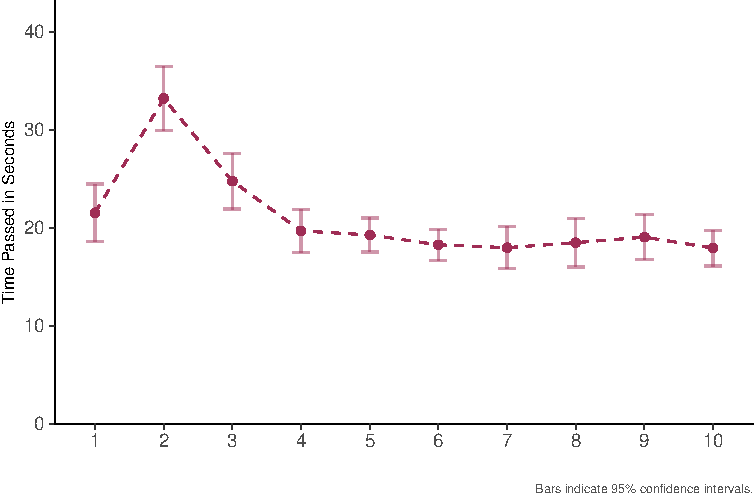
\includegraphics{/Users/hauke.roggenkamp/Documents/dev/coopUncertainty/analysis/reports/prettyReports/04_Analyses_files/figure-latex/plotTime-1.pdf}
\caption{Average Time Spent for each Contribution per Round.}
\end{figure}

Figure 4 illustrates the time participants needed to make each of their
contributions during the replication. One can see that the initial as
well as most of the other contributions take about 20 seconds of time.
Interestingly, the second contribution takes (on average) about 50\%
more time than the first one - presumably because this is the first time
participants' learn their respective group members' actions. The third
contribution is a little faster and all subsequent contributions
stabilize at 19 seconds.

Given that no participant dropped out after answering the comprehension
questions correctly and given that participants need less than 20
seconds to make their contributions, more than 10 rounds are feasible.

\hypertarget{sample-properties}{%
\section{Sample Properties}\label{sample-properties}}

\% Table created by stargazer v.5.2.2 by Marek Hlavac, Harvard
University. E-mail: hlavac at fas.harvard.edu \% Date and time: Tue, Feb
01, 2022 - 13:44:37

\begin{table}[!htbp] \centering 
  \caption{} 
  \label{} 
\begin{tabular}{@{\extracolsep{5pt}}lccccccc} 
\\[-1.8ex]\hline 
\hline \\[-1.8ex] 
Statistic & \multicolumn{1}{c}{N} & \multicolumn{1}{c}{Mean} & \multicolumn{1}{c}{St. Dev.} & \multicolumn{1}{c}{Min} & \multicolumn{1}{c}{Pctl(25)} & \multicolumn{1}{c}{Pctl(75)} & \multicolumn{1}{c}{Max} \\ 
\hline \\[-1.8ex] 
gender & 116 & 0.526 & 0.501 & 0 & 0 & 1 & 1 \\ 
age & 116 & 35.767 & 15.663 & 9 & 24 & 49.2 & 73 \\ 
switching\_row & 78 & 6.154 & 2.151 & 1.000 & 6.000 & 7.000 & 12.000 \\ 
education & 116 & 6.241 & 0.966 & 3 & 6 & 7 & 8 \\ 
donation & 116 & 0.931 & 1.672 & 0.000 & 0.000 & 1.000 & 11.050 \\ 
pq01 & 116 & 4.302 & 1.144 & 1 & 3.8 & 5 & 6 \\ 
pq02 & 116 & 2.681 & 1.702 & 0 & 1 & 4 & 6 \\ 
pq03 & 116 & 3.759 & 1.184 & 1 & 3 & 5 & 6 \\ 
pq04 & 116 & 1.853 & 1.551 & 0 & 1 & 2 & 6 \\ 
pq05 & 116 & 4.284 & 1.207 & 1 & 4 & 5 & 6 \\ 
pq06 & 116 & 3.672 & 1.525 & 0 & 3 & 5 & 6 \\ 
pq07 & 116 & 4.879 & 1.463 & 0 & 4 & 6 & 6 \\ 
pq08 & 116 & 4.647 & 1.385 & 1 & 4 & 6 & 6 \\ 
pq09 & 116 & 1.560 & 2.006 & 0 & 0 & 3 & 6 \\ 
pq10 & 116 & 3.009 & 1.639 & 0 & 2 & 4 & 6 \\ 
pq11 & 116 & 3.586 & 1.358 & 0 & 3 & 5 & 6 \\ 
pq12 & 116 & 3.914 & 1.564 & 0 & 3 & 5 & 6 \\ 
pq13 & 116 & 3.836 & 1.480 & 0 & 3 & 5 & 6 \\ 
pq14 & 116 & 4.241 & 1.618 & 0 & 3 & 6 & 6 \\ 
\hline \\[-1.8ex] 
\end{tabular} 
\end{table}

\begin{table}[!htbp] \centering 
  \caption{} 
  \label{} 
\begin{tabular}{@{\extracolsep{5pt}}lcccc} 
\\[-1.8ex]\hline 
\hline \\[-1.8ex] 
 & \multicolumn{4}{c}{\textit{Dependent variable:}} \\ 
\cline{2-5} 
 & female & age & risk & donations \\ 
\hline \\[-1.8ex] 
 Replication & 0.15$^{**}$ & 5.04$^{***}$ & $-$0.28 & 0.25 \\ 
  & (0.07) & (1.65) & (0.27) & (0.23) \\ 
  & & & & \\ 
 Constant & 0.38$^{***}$ & 30.73$^{***}$ & 6.44$^{***}$ & 0.68$^{***}$ \\ 
  & (0.05) & (1.23) & (0.19) & (0.17) \\ 
  & & & & \\ 
\hline \\[-1.8ex] 
Observations & 208 & 208 & 165 & 208 \\ 
R$^{2}$ & 0.02 & 0.04 & 0.01 & 0.01 \\ 
Residual Std. Error & 0.50 & 11.83 & 1.76 & 1.66 \\ 
\hline 
\hline \\[-1.8ex] 
\textit{Note:}  & \multicolumn{4}{r}{$^{*}$p$<$0.1; $^{**}$p$<$0.05; $^{***}$p$<$0.01} \\ 
\end{tabular} 
\end{table}

\begin{table}[!htbp] \centering 
  \caption{} 
  \label{} 
\begin{tabular}{@{\extracolsep{5pt}}lccccc} 
\\[-1.8ex]\hline 
\hline \\[-1.8ex] 
 & \multicolumn{5}{c}{\textit{Dependent variable:}} \\ 
\cline{2-6} 
 & quick thinker & easily offended & very satisfied & very dependent & generally happy \\ 
\hline \\[-1.8ex] 
 Replication & $-$0.77$^{***}$ & $-$1.03$^{***}$ & $-$1.23$^{***}$ & $-$0.94$^{***}$ & $-$1.36$^{***}$ \\ 
  & (0.17) & (0.23) & (0.17) & (0.20) & (0.16) \\ 
  & & & & & \\ 
 Constant & 5.08$^{***}$ & 3.71$^{***}$ & 4.99$^{***}$ & 2.79$^{***}$ & 5.64$^{***}$ \\ 
  & (0.13) & (0.17) & (0.13) & (0.15) & (0.12) \\ 
  & & & & & \\ 
\hline \\[-1.8ex] 
Observations & 208 & 208 & 208 & 208 & 208 \\ 
R$^{2}$ & 0.09 & 0.09 & 0.21 & 0.09 & 0.26 \\ 
Residual Std. Error & 1.20 & 1.66 & 1.21 & 1.46 & 1.15 \\ 
\hline 
\hline \\[-1.8ex] 
\textit{Note:}  & \multicolumn{5}{r}{$^{*}$p$<$0.1; $^{**}$p$<$0.05; $^{***}$p$<$0.01} \\ 
\end{tabular} 
\end{table}

\begin{table}[!htbp] \centering 
  \caption{} 
  \label{} 
\begin{tabular}{@{\extracolsep{5pt}}lccccc} 
\\[-1.8ex]\hline 
\hline \\[-1.8ex] 
 & \multicolumn{5}{c}{\textit{Dependent variable:}} \\ 
\cline{2-6} 
 & work important & family important & friends important & religion important & politics important \\ 
\hline \\[-1.8ex] 
 Replication & $-$1.04$^{***}$ & $-$0.61$^{***}$ & $-$1.30$^{***}$ & $-$0.87$^{***}$ & $-$0.69$^{***}$ \\ 
  & (0.20) & (0.21) & (0.18) & (0.26) & (0.22) \\ 
  & & & & & \\ 
 Constant & 4.72$^{***}$ & 5.49$^{***}$ & 5.95$^{***}$ & 2.43$^{***}$ & 3.70$^{***}$ \\ 
  & (0.15) & (0.16) & (0.13) & (0.20) & (0.16) \\ 
  & & & & & \\ 
\hline \\[-1.8ex] 
Observations & 208 & 208 & 208 & 208 & 208 \\ 
R$^{2}$ & 0.11 & 0.04 & 0.20 & 0.05 & 0.05 \\ 
Residual Std. Error & 1.46 & 1.51 & 1.28 & 1.88 & 1.58 \\ 
\hline 
\hline \\[-1.8ex] 
\textit{Note:}  & \multicolumn{5}{r}{$^{*}$p$<$0.1; $^{**}$p$<$0.05; $^{***}$p$<$0.01} \\ 
\end{tabular} 
\end{table}

\begin{table}[!htbp] \centering 
  \caption{} 
  \label{} 
\begin{tabular}{@{\extracolsep{5pt}}lcccc} 
\\[-1.8ex]\hline 
\hline \\[-1.8ex] 
 & \multicolumn{4}{c}{\textit{Dependent variable:}} \\ 
\cline{2-5} 
 & most people trusted & hard work better & government responsible & incomes equal \\ 
\hline \\[-1.8ex] 
 Replication & $-$0.28 & $-$1.52$^{***}$ & $-$0.48$^{**}$ & 0.42$^{*}$ \\ 
  & (0.19) & (0.21) & (0.20) & (0.23) \\ 
  & & & & \\ 
 Constant & 3.87$^{***}$ & 5.43$^{***}$ & 4.32$^{***}$ & 3.83$^{***}$ \\ 
  & (0.14) & (0.16) & (0.15) & (0.17) \\ 
  & & & & \\ 
\hline \\[-1.8ex] 
Observations & 208 & 208 & 208 & 208 \\ 
R$^{2}$ & 0.01 & 0.20 & 0.03 & 0.02 \\ 
Residual Std. Error & 1.36 & 1.52 & 1.42 & 1.63 \\ 
\hline 
\hline \\[-1.8ex] 
\textit{Note:}  & \multicolumn{4}{r}{$^{*}$p$<$0.1; $^{**}$p$<$0.05; $^{***}$p$<$0.01} \\ 
\end{tabular} 
\end{table}

\begin{table}[!htbp] \centering 
  \caption{} 
  \label{} 
\begin{tabular}{@{\extracolsep{5pt}}lcccc} 
\\[-1.8ex]\hline 
\hline \\[-1.8ex] 
 & \multicolumn{4}{c}{\textit{Dependent variable:}} \\ 
\cline{2-5} 
 & \multicolumn{2}{c}{Wealth} & \multicolumn{2}{c}{Gini} \\ 
\hline \\[-1.8ex] 
 female & $-$30.63 & $-$65.02 & 0.02 & 0.02 \\ 
  & (88.07) & (83.80) & (0.03) & (0.03) \\ 
  & & & & \\ 
 age & 7.05$^{*}$ & 9.00$^{**}$ & $-$0.001 & $-$0.001 \\ 
  & (3.82) & (3.60) & (0.001) & (0.001) \\ 
  & & & & \\ 
 risk & 27.21 & 10.98 & $-$0.01 & $-$0.01 \\ 
  & (22.65) & (19.45) & (0.01) & (0.01) \\ 
  & & & & \\ 
 quick thinker & $-$55.19 &  & 0.02 &  \\ 
  & (45.52) &  & (0.02) &  \\ 
  & & & & \\ 
 easily offended & $-$26.52 &  & 0.01 &  \\ 
  & (31.48) &  & (0.01) &  \\ 
  & & & & \\ 
 very satisfied & $-$2.62 &  & 0.001 &  \\ 
  & (42.60) &  & (0.02) &  \\ 
  & & & & \\ 
 very dependent & $-$22.41 &  & 0.0003 &  \\ 
  & (30.47) &  & (0.01) &  \\ 
  & & & & \\ 
 generally happy & 70.06 &  & 0.004 &  \\ 
  & (42.99) &  & (0.02) &  \\ 
  & & & & \\ 
 work important & $-$64.01 &  & $-$0.01 &  \\ 
  & (39.13) &  & (0.02) &  \\ 
  & & & & \\ 
 family important & 11.99 &  & $-$0.01 &  \\ 
  & (38.05) &  & (0.01) &  \\ 
  & & & & \\ 
 friends important & $-$24.05 &  & $-$0.004 &  \\ 
  & (37.94) &  & (0.01) &  \\ 
  & & & & \\ 
 religion important & $-$20.48 &  & 0.02$^{*}$ &  \\ 
  & (26.15) &  & (0.01) &  \\ 
  & & & & \\ 
 politics important & 86.94$^{***}$ &  & $-$0.01 &  \\ 
  & (30.79) &  & (0.01) &  \\ 
  & & & & \\ 
 most people trusted & $-$0.49 &  & $-$0.001 &  \\ 
  & (31.94) &  & (0.01) &  \\ 
  & & & & \\ 
 hard work better & 35.38 &  & $-$0.03$^{*}$ &  \\ 
  & (34.46) &  & (0.01) &  \\ 
  & & & & \\ 
 government responsible & $-$47.38 &  & $-$0.03$^{*}$ &  \\ 
  & (39.54) &  & (0.02) &  \\ 
  & & & & \\ 
 incomes equal & $-$9.13 &  & 0.01 &  \\ 
  & (33.79) &  & (0.01) &  \\ 
  & & & & \\ 
 Constant & 278.16 & 100.12 & 0.39$^{***}$ & 0.28$^{***}$ \\ 
  & (377.35) & (180.67) & (0.14) & (0.07) \\ 
  & & & & \\ 
\hline \\[-1.8ex] 
Observations & 78 & 78 & 78 & 78 \\ 
R$^{2}$ & 0.28 & 0.10 & 0.21 & 0.02 \\ 
Residual Std. Error & 357.69 & 360.58 & 0.14 & 0.14 \\ 
\hline 
\hline \\[-1.8ex] 
\textit{Note:}  & \multicolumn{4}{r}{$^{*}$p$<$0.1; $^{**}$p$<$0.05; $^{***}$p$<$0.01} \\ 
 & \multicolumn{4}{r}{Robust standard errors in parentheses, clustered by group ID.} \\ 
\end{tabular} 
\end{table}

\hypertarget{hamburg-how-do-students-compare-to-non-students}{%
\section{Hamburg: How do Students compare to
non-Students?}\label{hamburg-how-do-students-compare-to-non-students}}

This section considers the replication data only. Doing so, we'll
exploit the circumstance that we recruited from both the convenience or
``student'' sample as well as the non-convenience sample \emph{(Hamburg
Panel)} and analyze the differences between the two.

\begin{table}[!htbp] \centering 
  \caption{} 
  \label{} 
\begin{tabular}{@{\extracolsep{5pt}}lcc} 
\\[-1.8ex]\hline 
\hline \\[-1.8ex] 
Statistic & Students & HH.panel \\ 
\hline \\[-1.8ex] 
Mean & 10.172 & 9.827 \\ 
Median & 10 & 10.000 \\ 
St. Dev. & 6.470 & 6.233 \\ 
Max & 20 & 20.000 \\ 
Min & 0 & 0.000 \\ 
N & 64 & 52 \\ 
\hline \\[-1.8ex] 
\end{tabular} 
\end{table}

We start by looking at the initial contributions. As Table 5
illustrates, there is no difference in averages, standard deviation or
the range. The two-sided rank sum test (comparing differences between
data sources) yields a p-Value of 0.8902 for the mean contribution in
first round of the game.

While the initial contributions are on average quite similar between the
two sample, the subsequent contributions differ. In both absolute and
relative terms, the Hamburg-Panel tends to contribute more than the
student sample as the following Figure shows.

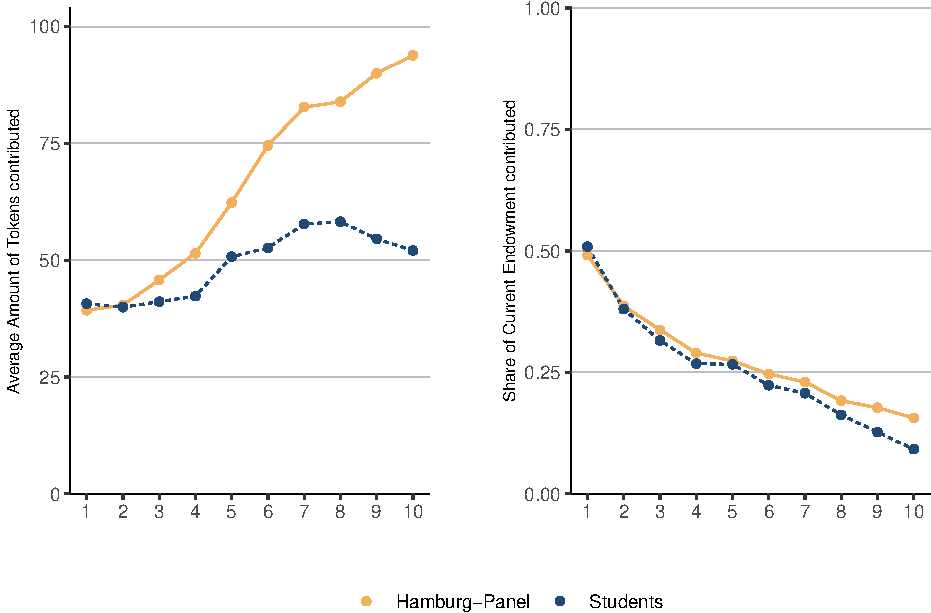
\includegraphics{/Users/hauke.roggenkamp/Documents/dev/coopUncertainty/analysis/reports/prettyReports/04_Analyses_files/figure-latex/sampleContributions-1.pdf}

Differences in contributions lead to differences in wealth. The
Hamburg-Panel therefore earned more during the public goods game than
the student sample. This can be seen in the following figure as well as
in the subsequent table:

\begin{figure}
\centering
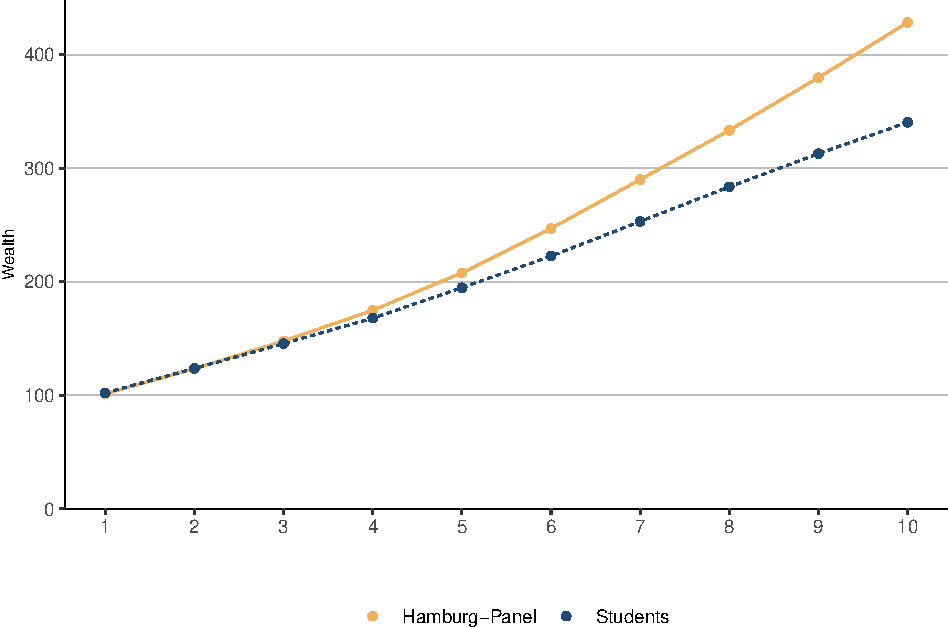
\includegraphics{/Users/hauke.roggenkamp/Documents/dev/coopUncertainty/analysis/reports/prettyReports/04_Analyses_files/figure-latex/sampleStock-1.pdf}
\caption{Average wealth over time across samples.}
\end{figure}





\newpage
\singlespacing 
\bibliography{../biblio.bib}

\end{document}